%CaseQuad
\todo[inline]{Start by motivating the example as something more than a dumb system. E.g. "Air traffic control offers many opportunities for automation to allow a more efficient and safer landing patterns. The constraints of air traffic control are complex and contain many safety rules. In this example we express these rules in MTL and demonstrate how the smoothed robustness is used to generate control strategies for safely and robustly landing two quadrotors. The proposed approach outperforms Simulated Annealing and gradient descent on the non-smooth robustness."
	
	Then you give the details below}
1. We take a quad-rotor model with linearized dynamics around hover, similar to those used in \cite{}. The case study involves centralized control of two quad-rotors, with operational objectives given as an MTL specification, and a constrained air-space.

1.b. Give model, constraints, specification. Shrinking horizon (fixing history) approach applicable (cite Vasu paper)

2. With the given specification, standard control approaches involving polyhedral constraints are hard to apply because of the temporal aspect of the eventually operator involved. While the two (if-then) altitude rules in the specification can be coded as polyhedral constraints on the set, it would result in a non-convex constraint set for positions. Similarly, the minimum distance between two quad-rotors can also be moved to the constraints but would result in another non-convex constraint if we choose to do so. In our formulation, the non-convexity remains in the cost-function while the constraints are linear.

3. For simulation purposes, we use obtain 3 initial trajectories (via solving different linear programs) from the given initial state to the terminal (landing) set. These three trajectories, each of which has negative robustness (i.e. does not satisfy the given specification), serve as three different initial solutions to A) Our approach B) SQP using the actual robustness function as the cost, C) Simulated Annealing with the actual robustness function as the cost. This multi-start approach can be used in practice when there is a fast initial trajectory generator available.

3.b. parameters for simulation annealing and citation for it.

4. Fig shows the initial trajectories for both the quadrotors in the given air-space. Fig. shows the three trajectories obtained after applying our control method, with the three initial trajectories as starting points for the optimization, respectively. 

5. Table shows for the three trajectories, initial robustness, robustness for trajectory obtained via the three methods (and the approximate robustness when applicable). In addition, we also tested out simulated annealing with the smooth robustness function in the cost (with the first initial trajectory), resulting in a trajectory with a final cost of blah (approximate robustness of blah).



\begin{figure}[t]
\centering
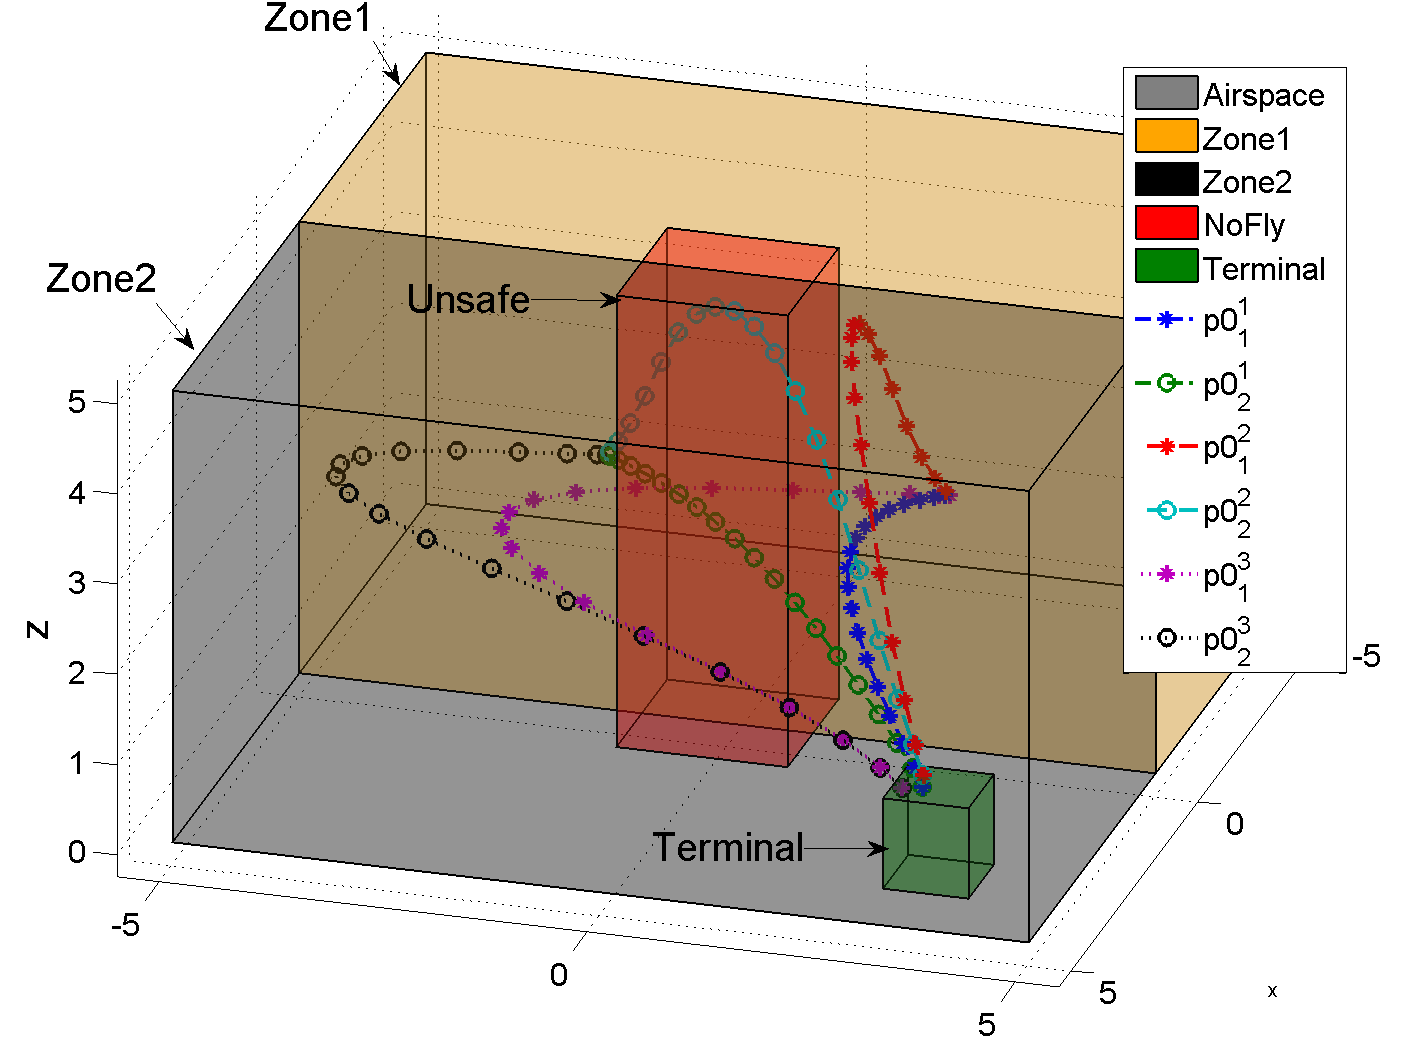
\includegraphics[width=0.49\textwidth]{figures/QuadInitTrajs_scissored}
\caption{The airspace with the corresponding sets, and initial trajectories for the two quad-rotors. Note, all 3 initial trajectories violate the specification. Here, $p0_{i}^j$ refers to the positions of the $i^{th}$ initial trajectory for the $j^{th}$ quadrotor.}
\label{fig:quad_init}
\end{figure}

\begin{figure}[t]
\centering
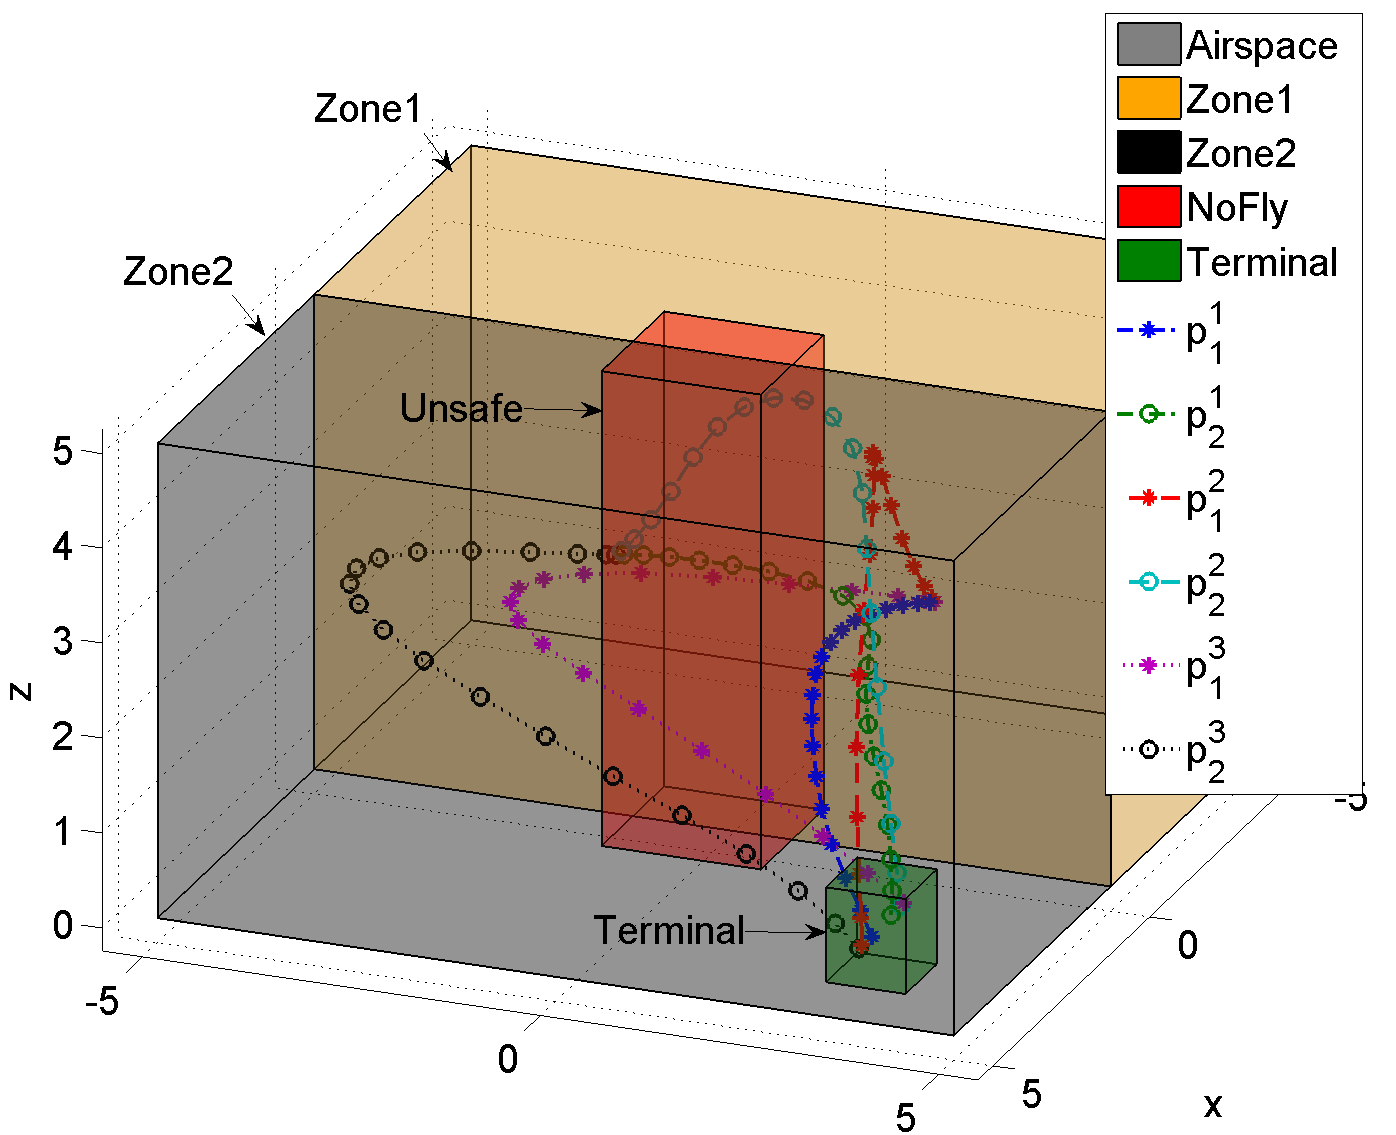
\includegraphics[width=0.49\textwidth]{figures/QuadTrajs_scissored}
\caption{ Trajectories obtained via SQP on smooth robustness, with three different initial trajectories acting as initial solutions for the SQP. Note, all 3 trajectories satisfy $\Psi$. Here, $p_{i}^j$ refers to the positions of the $i^{th}$ initial trajectory for the $j^{th}$ quadrotor.}
\label{fig:quad_init}
\end{figure}
